\section{Performance Evaluation}
\label{sec:evaluation}

This section evaluates SSHv2, SSH3, and Mosh across three interactive AI agent workloads: command completion with small output (W1), large output delivery (W2), and interactive keystroke latency (W3, in single-pane and five-pane tmux layouts). Measurements were conducted under four network conditions, namely VPN (Tailscale over the public Internet) and three controlled tc/netem profiles labeled Low, Medium, and High. The evaluation also reports two cross-cutting metrics that apply to all workloads: session establishment latency, captured before any workload iteration begins, and output completeness, defined as the percentage of expected bytes received by the client. Table~\ref{tab:samples} summarizes the number of collected samples for each measurement case. We use these samples as the basis for the statistical analysis reported in the following subsections.

\begin{table*}[t]
\centering
\caption{Summary of collected samples in the measurement campaign.}
\label{tab:samples}
\begin{tabular}{p{3.2cm}p{4.6cm}p{2.6cm}p{2.8cm}p{3.6cm}}
\hline
\textbf{Measurement case} & \textbf{Scenario / configuration} & \textbf{Protocol(s)} & \textbf{Sampling unit} & \textbf{Collected samples} \\
\hline
Session establishment & VPN (Tailscale over the public Internet), Low, Medium, and High tc/netem profiles. & SSHv2, SSH3, Mosh & One session-setup attempt (process spawn to first prompt) & 60 attempts per protocol in VPN; 18 attempts per protocol in each of Low, Medium, and High. \\
\hline
Command completion (W1) & Four small-output commands ($\leq$1\,KB): \texttt{ls}, \texttt{df~-h}, \texttt{grep~-n~root~/etc/passwd}, \texttt{git~status}, under all four scenarios. & SSHv2, SSH3, Mosh & One command-completion measurement & 10 sessions $\times$ 100 samples per command, post-warmup, aggregated across the four commands. \\
\hline
Large output delivery (W2) & Three large-output commands (tens of KB): \texttt{find~/}, \texttt{ps~aux}, \texttt{docker~logs}, under all four scenarios; 20\,s per-sample timeout. & SSHv2, SSH3, Mosh & One command-completion measurement & 10 sessions $\times$ 100 samples per command for SSHv2 and SSH3; reduced for Mosh due to timeouts (e.g., 53 valid samples in High). \\
\hline
Interactive keystroke (W3) & Tmux probe stream in two layouts: single-pane and five-pane (background output on the four non-probe panes), under all four scenarios. & SSHv2, SSH3, Mosh & One typed character (keystroke-to-echo measurement) & 3,000 keystrokes per protocol in VPN; 900 keystrokes per protocol in each of Low, Medium, and High, for each layout. \\
\hline
Output completeness & Derived from W1 (lightweight) and W2 (heavy-output) captured outputs, compared against a reference output via direct SSH execution. & SSHv2, SSH3, Mosh & One \texttt{received\_pct} value per command-completion sample & Same population as W1 and W2 above. \\
\hline
\end{tabular}
\end{table*}

\subsection{Session Establishment Latency}
\label{subsec:session-setup}

We compare SSHv2, SSH3, and Mosh on session establishment latency across four network scenarios: VPN (Tailscale over the public Internet) and three controlled tc/netem profiles labeled Low, Medium, and High. For each (protocol, scenario) pair, we measure the time from client process spawn to the first interactive shell prompt, isolating pure transport and authentication overhead before any workload traffic. We collect 60 attempts per protocol in VPN and 18 attempts per protocol in each tc/netem profile (see Table~\ref{tab:samples}), and report the mean.

\begin{figure}[t]
    \centering
    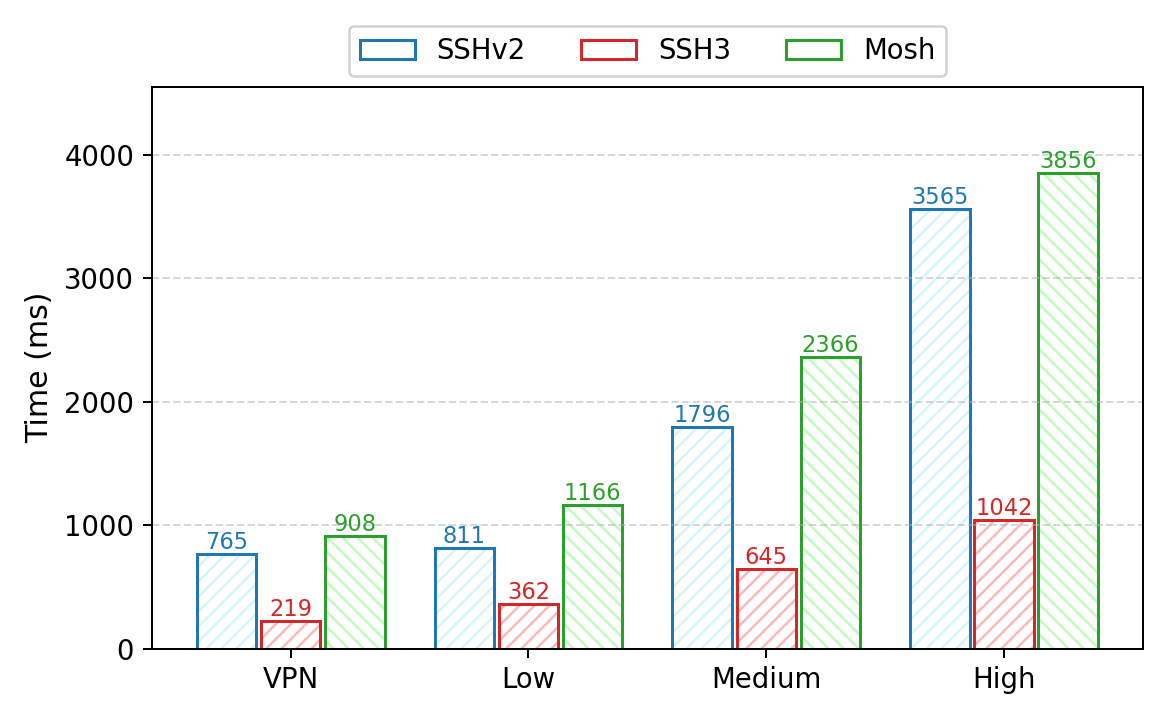
\includegraphics[width=\columnwidth]{figs/session_setup_bar.png}
    \caption{Mean session establishment latency across four network scenarios.}
    \label{fig:session-setup}
\end{figure}

Figure~\ref{fig:session-setup} reports the mean session-setup time. SSH3 consistently achieves the lowest setup latency across all scenarios. For example, in the VPN scenario, SSH3 establishes a session in 219\,ms on average, while SSHv2 requires 765\,ms (a 71\% reduction) and Mosh requires 908\,ms (a 76\% reduction). The same trend holds under tc/netem impairment: in the High scenario (RTT $\approx$200\,ms, 3\% loss), SSH3 completes setup in 1042\,ms on average, compared to 3565\,ms for SSHv2 and 3856\,ms for Mosh.

This difference is a direct consequence of protocol design. SSH3 uses QUIC's 1-RTT handshake, which combines transport setup and cryptographic key exchange into a single round trip. SSHv2, by contrast, requires a TCP three-way handshake followed by SSH key exchange and authentication (2--3 RTTs). Mosh incurs the highest cost because it first completes a full SSHv2 session to bootstrap the UDP-based SSP channel, adding an extra round trip on top of the SSH handshake.

\subsection{Command Completion Latency (W1)}
\label{subsec:w1-results}

W1 measures the end-to-end completion latency of short commands that produce small output ($\leq$1\,KB). The four commands evaluated are \texttt{ls}, \texttt{df~-h}, \texttt{grep~-n~root~/etc/passwd} (referred to as \texttt{grep} hereafter), and \texttt{git~status}. The W1 rows of Table~\ref{tab:workload-latency} report the mean across all four commands, computed by first averaging per command and then averaging across commands. Table~\ref{tab:workload-latency} also consolidates the W2 and W3 results discussed in the following subsections.

\begin{table}[t]
\centering
\caption{Mean latency (ms) for the three workloads across protocols and network scenarios. W1: small-output commands (\texttt{ls}, \texttt{df~-h}, \texttt{grep}, \texttt{git~status}). W2: large-output commands (\texttt{find~/}, \texttt{ps~aux}, \texttt{docker~logs}). W3: keystroke-to-echo latency in single-pane (1p) and five-pane (5p) tmux layouts. Bold marks the lowest value in each row.}
\label{tab:workload-latency}
\begin{tabular}{llrrr}
\hline
\textbf{Workload} & \textbf{Scenario} & \textbf{SSHv2} & \textbf{SSH3} & \textbf{Mosh} \\
\hline
\multirow{4}{*}{W1}
 & VPN     & 93.1  & \textbf{81.6}  & 97.0  \\
 & Low     & 97.3  & \textbf{92.9}  & 102.9 \\
 & Medium  & 194.9 & \textbf{176.2} & 197.1 \\
 & High    & 384.4 & \textbf{292.9} & 324.4 \\
\hline
\multirow{4}{*}{W2}
 & VPN     & 159.8           & \textbf{87.7}  & 96.8           \\
 & Low     & \textbf{432.0}  & 461.6          & 461.1          \\
 & Medium  & 1144.9          & 739.3          & \textbf{561.4} \\
 & High    & 2680.0          & 1384.7         & \textbf{709.6} \\
\hline
\multirow{4}{*}{W3-1p}
 & VPN     & 20.2  & 2.1   & \textbf{1.5}  \\
 & Low     & 26.1  & 29.3  & \textbf{2.6}  \\
 & Medium  & 116.7 & 112.0 & \textbf{13.2} \\
 & High    & 234.5 & 221.8 & \textbf{31.3} \\
\hline
\multirow{4}{*}{W3-5p}
 & VPN     & 23.9  & 9.4   & \textbf{1.2}  \\
 & Low     & 50.4  & 58.3  & \textbf{3.8}  \\
 & Medium  & 152.9 & 145.7 & \textbf{7.3}  \\
 & High    & 291.4 & 279.6 & \textbf{25.3} \\
\hline
\end{tabular}
\end{table}

For W1, SSH3 achieves the lowest mean completion latency across all four scenarios (Table~\ref{tab:workload-latency}, W1 rows). On the VPN scenario, SSH3 averages 81.6\,ms, a 12\% reduction over SSHv2 (93.1\,ms) and 16\% over Mosh (97.0\,ms). The advantage grows with impairment: under Medium, SSH3 averages 176.2\,ms versus 194.9\,ms for SSHv2 (10\% reduction) and 197.1\,ms for Mosh (11\% reduction); under High, SSH3 reaches 292.9\,ms compared to 384.4\,ms for SSHv2 and 324.4\,ms for Mosh, a 24\% reduction relative to SSHv2 and 10\% relative to Mosh.

This pattern is again a direct consequence of protocol design. Each W1 command produces less than one kilobyte, so the entire response fits within a single congestion window and the dominant cost per command is the round-trip needed to ship the request and receive the prompt. SSH3's QUIC transport pipelines request bytes alongside the cryptographic handshake on the same round trip, whereas SSHv2 must wait for a separate TCP+SSH exchange before any command bytes can flow on each new request channel. The gap therefore tracks the network RTT: the higher the RTT, the larger the absolute time saved per command (e.g., 91\,ms saved over SSHv2 in High, versus 12\,ms in VPN).

Mosh, by contrast, shows no advantage on W1 despite its UDP-based design. SSP coalesces multiple terminal updates into a single frame to reduce wire traffic, but with sub-kilobyte outputs the entire response already arrives in one frame interval, leaving no redundant updates to discard. Mosh therefore inherits the underlying SSHv2 round-trip cost without recouping it through frame reduction, and trails both SSH3 and SSHv2 under VPN and Low. Under Medium and High, Mosh closes the gap to SSHv2 because SSP recovers from packet loss locally on the UDP channel, avoiding the TCP retransmission stalls that inflate SSHv2's tail; nonetheless, SSH3 remains uniformly the fastest choice for short request-response loops.

\subsection{Large Output Delivery Latency (W2)}
\label{subsec:w2-results}

W2 measures the completion latency of commands that produce larger output (tens of kilobytes). The three commands evaluated are \texttt{find~/}, \texttt{ps~aux}, and \texttt{docker~logs}. The W2 rows of Table~\ref{tab:workload-latency} report the mean across all three commands.

For W2, no single protocol dominates; the ranking shifts with network condition (Table~\ref{tab:workload-latency}, W2 rows). Under VPN, SSH3 is fastest (87.7\,ms), benefiting from QUIC's stream-multiplexed delivery. Under Low impairment, the three protocols converge (432--462\,ms), as the moderate RTT amortizes both QUIC's and TCP's per-byte overhead. Under Medium and High, however, Mosh's mean latency (561.4 and 709.6\,ms) is dramatically below SSHv2 (1144.9 and 2680.0\,ms) and SSH3 (739.3 and 1384.7\,ms). At High, SSHv2 is 3.8$\times$ slower and SSH3 is 2.0$\times$ slower than Mosh.

Mosh's apparent advantage is misleading. As shown in Section~\ref{subsec:output-completeness}, Mosh delivers only 2--6\% of the expected bytes for large-output commands because SSP discards intermediate terminal states. The benchmark therefore measures time-to-prompt for Mosh, not time-to-complete-output. SSH3's poor performance relative to SSHv2 under impairment also stands out: at High, SSH3 (1384.7\,ms) is slower than expected, likely reflecting the immaturity of QUIC implementations in SSH3 v0.1.7 (more conservative congestion control and per-stream framing overhead for sustained bulk transfers).

\subsubsection{Failure rates}
SSHv2 and SSH3 achieve perfect reliability (0 failures across all scenarios and commands). Mosh exhibits significant failures for large-output commands: only 53 successful samples out of 300 attempts in the High scenario (82\% failure rate), and reduced effective sample counts (53--515 vs.\ 600--1200 for SSH/SSH3) across other scenarios.

\subsection{Output Completeness}
\label{subsec:output-completeness}

A key metric for AI agent workloads is whether the client receives the complete command output. Figure~\ref{fig:recv-pct} reports the mean percentage of expected output bytes received by the client (\texttt{received\_pct}), computed by comparing the captured output length against a reference collected via direct SSH execution.

\begin{figure}[t]
    \centering
    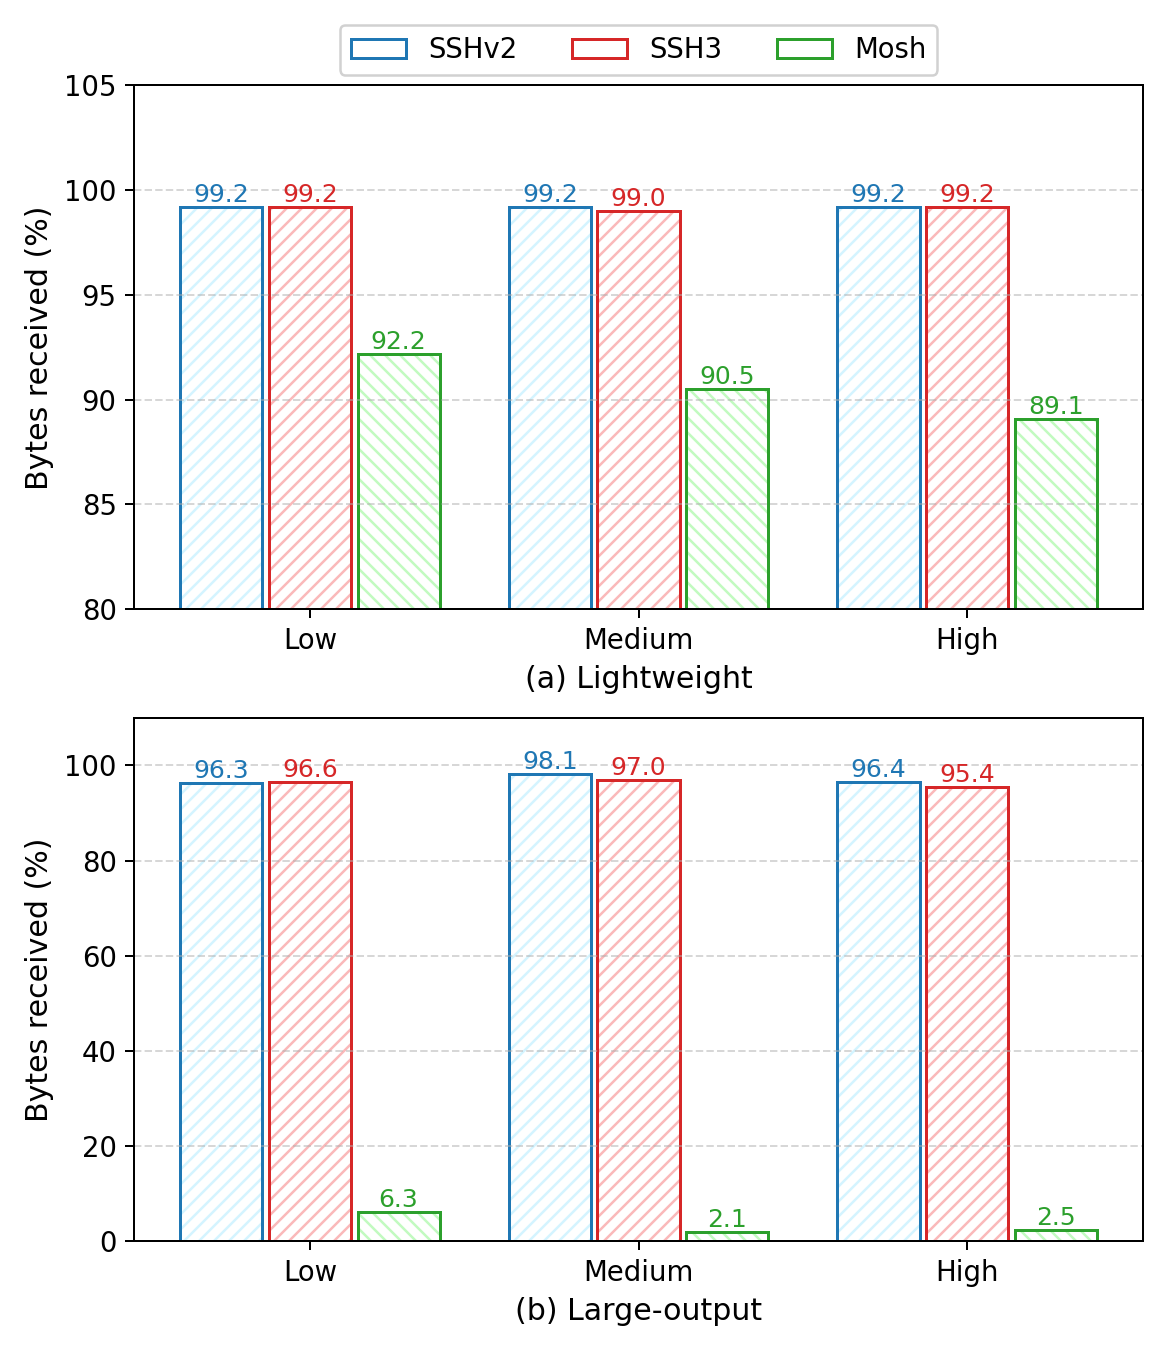
\includegraphics[width=\columnwidth]{figs/recv_pct_bar.png}
    \caption{Output completeness (percentage of expected bytes received).}
    \label{fig:recv-pct}
\end{figure}

SSHv2 and SSH3 both maintain high output completeness across all scenarios ($\geq$95\%), confirming that their byte-stream transport reliably delivers the full command output regardless of network conditions.

Mosh presents a fundamentally different picture. For heavy-output commands, Mosh delivers only 2--6\% of the expected output across all scenarios. Even for lightweight commands producing less than 1\,KB, Mosh's completeness drops to 89--92\%. This is not a failure mode but an inherent property of SSP: it synchronizes the terminal display state rather than the output byte stream. When multiple screen updates arrive within a single frame interval ($\sim$60\,ms), only the final state is transmitted.

For interactive human users, this trade-off is acceptable---the user sees the final result. For AI agents that must parse intermediate output (e.g., extracting specific lines from \texttt{ps~aux} or parsing directory listings from \texttt{find}), Mosh's frame-skipping behavior means the agent operates on incomplete data. This can lead to incorrect parsing, missed information, and cascading errors in the agent's decision loop.

\subsection{Interactive Keystroke Latency (W3)}
\label{subsec:w3-results}

W3 measures keystroke-to-echo latency under interactive use. We script a tmux session that types characters at a steady cadence and timestamps the moment each character is rendered back. Two layouts are evaluated: a single pane (\texttt{w3}, 1-pane) and a five-pane split layout (\texttt{w3-5}, 5-pane), the latter representing a more demanding terminal multiplexing workload that forces frequent screen redraws across multiple regions. The W3-1p and W3-5p rows of Table~\ref{tab:workload-latency} report the mean keystroke latency for each layout.

Mosh dominates W3 across every scenario and layout, often by an order of magnitude (Table~\ref{tab:workload-latency}, W3 rows). Under the High scenario, Mosh keystroke latency stays at 25--31\,ms whereas SSHv2 reaches 234--291\,ms and SSH3 reaches 222--280\,ms (7--11$\times$ higher). The gap originates from SSP's local-echo and predictive rendering: keystrokes are echoed locally on the client and then reconciled with the authoritative server state asynchronously, so user-perceived latency is decoupled from network RTT. SSHv2 and SSH3 both round-trip every character to the remote pseudo-terminal before echoing, so their latency tracks RTT directly.

SSH3's QUIC transport offers a clear benefit only under the VPN scenario (2.1\,ms vs.\ 20.2\,ms for SSHv2 in 1-pane), where 0-RTT request shipping eliminates a round trip. Under impaired networks, SSH3 performs comparably to SSHv2 (e.g., 221.8\,ms vs.\ 234.5\,ms in High 1-pane), and is even slightly slower than SSHv2 under Low (29.3\,ms vs.\ 26.1\,ms in 1-pane), again pointing to the immaturity of QUIC stack tuning in the SSH3 implementation.

The five-pane layout amplifies redraw traffic and stresses the protocols differently. SSHv2 and SSH3 both incur 18--96\% additional latency moving from 1-pane to 5-pane, as each redraw must be transmitted over the network. Mosh, in contrast, shows negligible or even reduced 5-pane latency (e.g., 1.2\,ms vs.\ 1.5\,ms in VPN; 7.3\,ms vs.\ 13.2\,ms in Medium), because SSP coalesces multi-pane updates into a single terminal frame before transmission---additional panes do not multiply the wire workload. This confirms that for human-interactive use over impaired networks, especially with multi-pane layouts, Mosh remains the most responsive option.

\subsection{Key Takeaways}
\label{subsec:takeaways}

% TODO
